\documentclass[12pt,a4paper]{article}
\usepackage[utf8]{inputenc}
\usepackage{graphicx}
\usepackage{tikz}
\usetikzlibrary{fit}
\usepackage{lmodern}
\usepackage{sectsty}


\sectionfont{\color{cyan}}

\begin{document}
   \begin{titlepage}
      {\fontfamily{lmss}\selectfont
      	\centering
      	
\includegraphics[width=0.30\textwidth]{logo.png}\par\vspace{1cm}
      	{\LARGE Capstone Project Demo 1 \par}
      	\vspace{0.25cm}
      	{\huge\bfseries \color{cyan}System Requirements and Design Document\par}
      	\vspace{1cm}
      	{\Large\textit{by} Brute Force\par}
         \vspace{0.25cm}
         \begin{tikzpicture}
            \node [inner sep=0pt,,outer sep=0pt,clip,rounded corners=0.5cm] (pict) at (0,0) {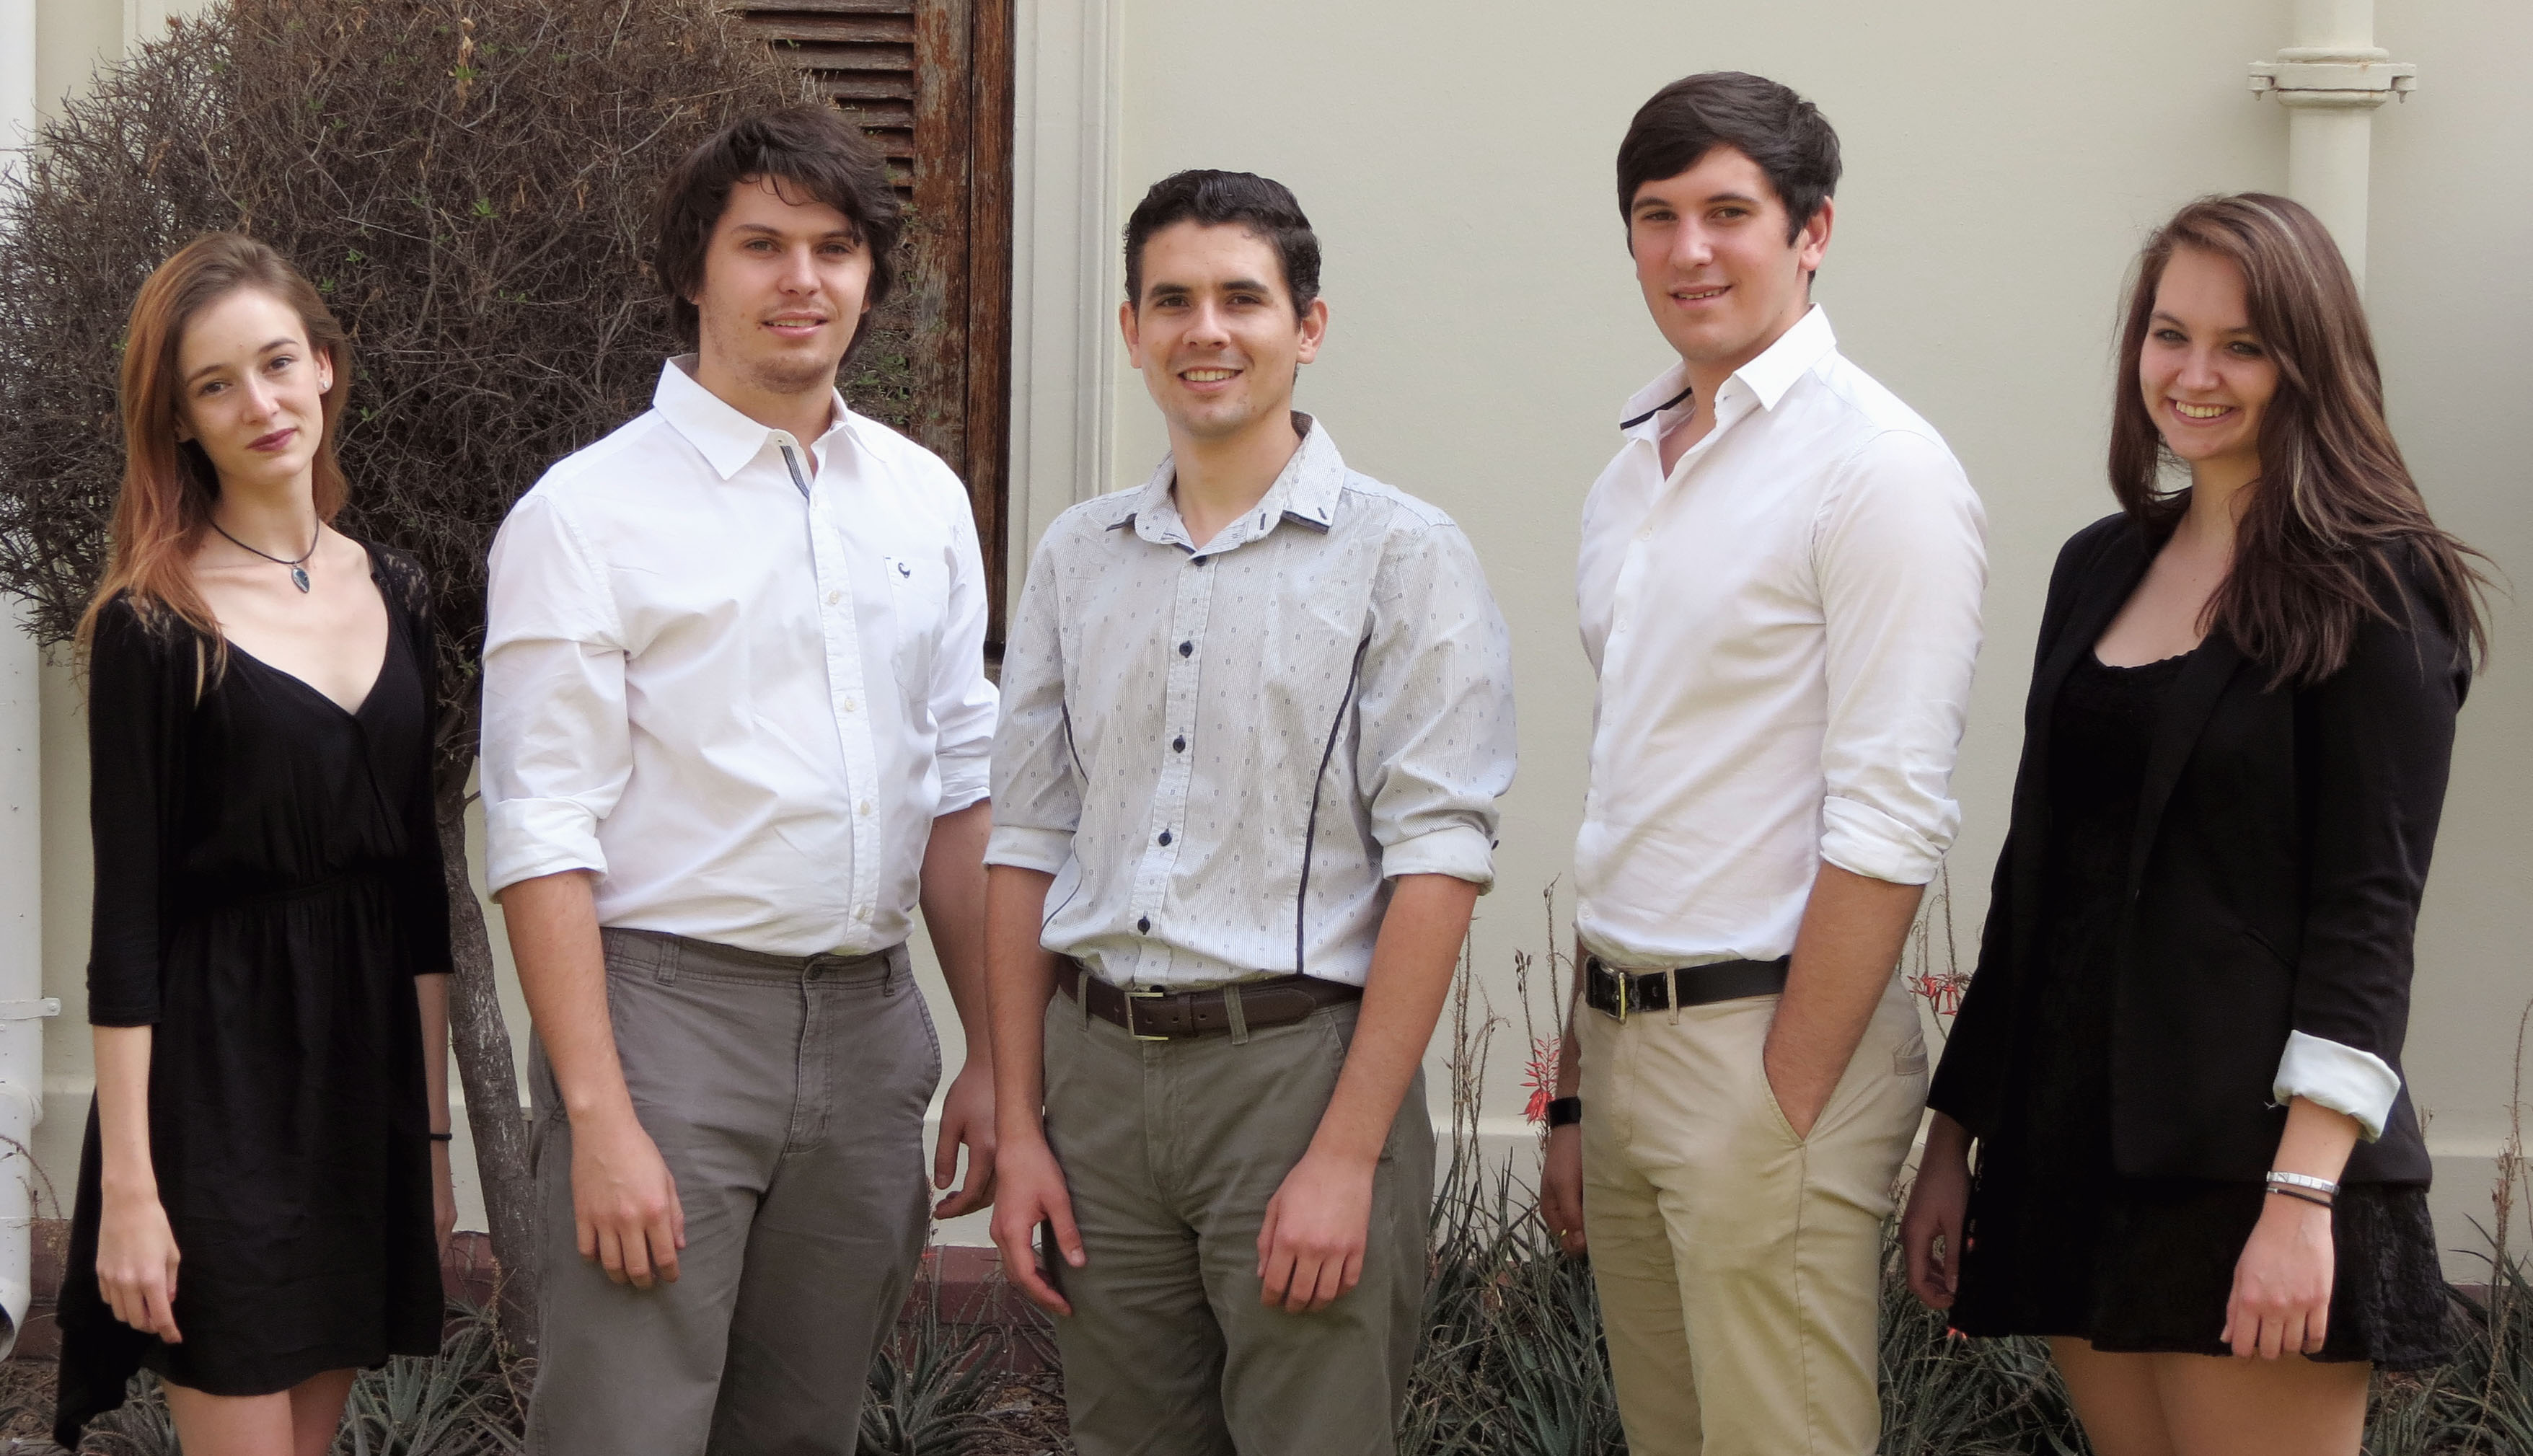
\includegraphics[width=0.9\textwidth]{team.jpg}};
            \node[fit=(pict),rounded corners=.55cm,inner sep=2pt]{};
         \end{tikzpicture}

         \par\vspace{1cm}
         \date{}
         \author{}
         \title{}
         \centering
         \textbf{Authors:}\\
         Mia Gerber\\
         Matthew Perry\\
         Wanrick Willemse\\
         Duart Breedt\\
         Linda Potgieter\\
      }
   \end{titlepage}
   \maketitle
   \tableofcontents
   \newpage

   \section{Introduction}
   	\subsection{Purpose}
		\paragraph{Application for splitting a restaurant bill between friends.}
		The application will be used as a utility in a social context to decrease the time it takes to work out how much everyone needs to contribute to a shared bill. 
		
   	\subsection{Scope}	
   	This project will essentially be divided into two phases, the first of which focuses heavily on user experience and the second accuracy.
		\paragraph{Phase One:}
		A multi-platform mobile application that users can send a photo of a bill to and receive an interactive interface generated from the data contained within that photo that they can then use to work out correct totals.
		\paragraph{Phase Two:}
		An artificial intelligence agent that has been trained to recognise text in a photo in a very specific way will be the backend mechanism that can be given any photo and will return a JSON object with the structure of that photo that can be parsed to create the interface in phase one. 
		
   	\subsection{Overview}
The goal of this document is to define a clear project scope that will be used to contain and guide coming deliverables as well as give clarity as to how our application will function as a system built up out of well-defined components.

   \section{Overall Description}
   	\subsection{System Interfaces}
   	
   	\subsection{User Interfaces}
   		
   	\subsection{Hardware Interfaces}
   	
   	\subsection{Software Interfaces}
   		% UML diagrams will go here
   	\subsection{Product Functions}
   		% Use cases could possibly be sensible here
	\subsection{User Characteristics}   	
   		% actor-system modelling
		Our application is being marketed as a "utility" and as such we won't be targeting a specific user, we want to appeal to as many people as possible because the type of person who visits a restaurant with friends is almost every person imaginable. With that said we will however assume our users to be literate in mobile technologies. A basic understanding of touch screen gestures and navigation between different screens will be assumed. We are making HCI (Human Computer Interaction) a major focus during development of our GUI and as such the aim is simplicity and usability without losing aesthetic appeal. 		
		
   	\subsection{Assumptions and Dependencies}

   \section{Specific Requirements}
	\subsection{External Interface Requirements}
	
	\subsection{Functional Requirements}
	
		\begin{enumerate}
				\item The system must be able to recognise text on a bill.
				\item The system must be able to correctly categorise the different "columns" of text into discrete structures that represent different information semantically (e.g. an item of food is not interpreted as a numeric amount)
				\item The system should consciously check whether it has correctly interpreted the bill and if it did not ask the user either for a higher quality photo or as a last resort give an error message. 
				\item The system should return all information gleaned from the OCR process as a JSON object of which the structure is known to the component that will be receiving the object.
			\end{enumerate}

			\begin{enumerate}
				\item The user interface provides a facility for both taking a photo and sending it to the server.
				\item The user interface provides a facility for starting a new session which will return a temporary session code which is shared with users who also have the application around the table.
				\item The user interface which is generated after interpretation of the bill (after the associated JSON object has been received) contains a  facility for choosing items to pay for and generates a running total as the user decides.
				\item All user that were added to the current session will receive the exact same interface and as such will be able to see which items are still available to be paid for and which are no longer available. (Asynchronous calls to the server will facilitate updating of the user interface)
			\end{enumerate}
		
	\subsection{Performance Requirements}
	
	\subsection{Design Constraints}
	
		\begin{itemize}
			\item Even though we will not be persisting any image data for longer than necessary the size of images being sent to the server is a constraint we will need to be conscious of, possible solutions will be cropping or simply reducing image quality by changing the image to only use black and white or a degree of grayscaling.
			\item The experience of the development team might influence the degree to which the artificial intelligence portion of this project comes to fruition.
			\item The possibility of getting the application to still be functional without internet access can become a design constraint later in development.
		\end{itemize}
	
	\subsection{Software System Attributes}
   
\end{document}
